\documentclass[10pt]{article}
\usepackage[letterpaper]{geometry}
\geometry{verbose,tmargin=1in,bmargin=1in,lmargin=1in,rmargin=1in}
\usepackage{setspace}
\usepackage{ragged2e}
\usepackage{color}
\usepackage{titlesec}
\usepackage{graphicx}
\usepackage{float}
\usepackage{mathtools}
\usepackage{amsmath}
\usepackage[font=small,labelfont=bf,labelsep=period]{caption}
\usepackage[english]{babel}
\usepackage{indentfirst}
\usepackage{array}
\usepackage{makecell}
\usepackage[usenames,dvipsnames]{xcolor}
\usepackage{multirow}
\usepackage{tabularx}
\usepackage{arydshln}
\usepackage{caption}
\usepackage{subcaption}
\usepackage{xfrac}
\usepackage{etoolbox}
\usepackage{cite}
\usepackage{url}
\usepackage{dcolumn}
\usepackage{hyperref}
\usepackage{courier}
\usepackage{esvect}
\usepackage{commath}
\usepackage{verbatim} % for block comments
\usepackage{enumitem}
\usepackage{hyperref} % for clickable table of contents
\usepackage{braket}
\usepackage{titlesec}
\usepackage{booktabs}
\usepackage{gensymb}
\usepackage{listings}
\usepackage{cancel}
\usepackage[mathscr]{euscript}
\lstset{
    frame=single,
    	basicstyle=\ttfamily\small,
    breaklines=true,
    postbreak=\raisebox{0ex}[0ex][0ex]{\ensuremath{\color{red}\hookrightarrow\space}}
}

% for circled numbers
\usepackage{tikz}
\newcommand*\circled[1]{\tikz[baseline=(char.base)]{
            \node[shape=circle,draw,inner sep=2pt] (char) {#1};}}

\newcommand{\beq}{\begin{equation}}
\newcommand{\eeq}{\end{equation}}
\newcommand{\beqa}{\begin{equation}\begin{aligned}}
\newcommand{\eeqa}{\end{aligned}\end{equation}}

\titleclass{\subsubsubsection}{straight}[\subsection]

% define new command for triple sub sections
\newcounter{subsubsubsection}[subsubsection]
\renewcommand\thesubsubsubsection{\thesubsubsection.\arabic{subsubsubsection}}
\renewcommand\theparagraph{\thesubsubsubsection.\arabic{paragraph}} % optional; useful if paragraphs are to be numbered

\titleformat{\subsubsubsection}
  {\normalfont\normalsize\bfseries}{\thesubsubsubsection}{1em}{}
\titlespacing*{\subsubsubsection}
{0pt}{3.25ex plus 1ex minus .2ex}{1.5ex plus .2ex}

\makeatletter
\renewcommand\paragraph{\@startsection{paragraph}{5}{\z@}%
  {3.25ex \@plus1ex \@minus.2ex}%
  {-1em}%
  {\normalfont\normalsize\bfseries}}
\renewcommand\subparagraph{\@startsection{subparagraph}{6}{\parindent}%
  {3.25ex \@plus1ex \@minus .2ex}%
  {-1em}%
  {\normalfont\normalsize\bfseries}}
\def\toclevel@subsubsubsection{4}
\def\toclevel@paragraph{5}
\def\toclevel@paragraph{6}
\def\l@subsubsubsection{\@dottedtocline{4}{7em}{4em}}
\def\l@paragraph{\@dottedtocline{5}{10em}{5em}}
\def\l@subparagraph{\@dottedtocline{6}{14em}{6em}}
\makeatother


\setcounter{secnumdepth}{4}
\setcounter{tocdepth}{4}
\begin{document}

\title{MATH 228b: HW6 1a,b,c, 2 bc,d,e, c}
\author{April Novak}

\maketitle

\section{}

\section{}

\textbf{(a)}

The first part of this question develops a Gauss-Seidel solver given a matrix system \(Au=b\) for an initial guess \(u_0\). This method is very similar to the Jacobi method, where instead of solving the time-independent problem of interest, we insert a time derivative term and iterate until the solution converges to a steady-state result (with the assumption that this steady-state result is therefore also equivalent to the solution to the problem with no time derivative at all). Gauss-Seidel differs from the Jacobi method in that the most recent iterate is used to perform the update. The code developed for this section is included in the Appendix.

\textbf{(b)}

This question solves the Poisson equation using the multigrid method. The first step is a modification to Professor Persson's {\tt pmesh} function (which I assume is okay because we were told for assignment 3 that we could use his function moving forward to avoid points being lost across multiple assignments) such that it outputs the {\tt data} structured array data structure containing {\tt data.p}, {\tt data.t}, and {\tt data.e} members. This is performed by manipulating the contents of the original {\tt pmesh} function, so make sure to use the {\tt pmesh} function that I submit with this assignment! This edited function is included in the Appendix.

In order to simplify the multigrid method, which relies upon repeated applications of interpolation (expanding a coarse solution to a finer mesh) and reduction (removing elements from a solution to coarsen), these interpolation and reduction matrices are pre-computed.















\begin{comment}
\begin{figure}[H]
\centering
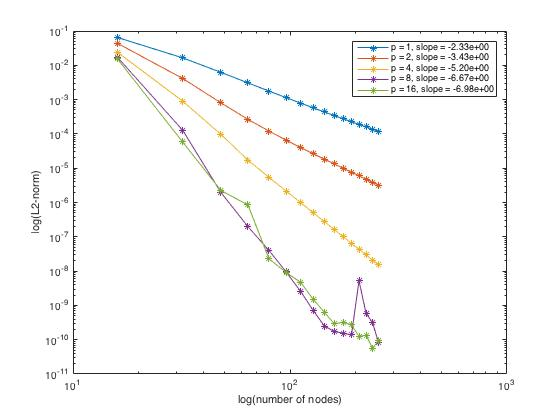
\includegraphics[width=0.8\textwidth]{figures/errors_raw.jpg}
\caption{\(L^2\) norm as a function of the number of nodes.}
\label{fig:errors_raw}
\end{figure}
\end{comment}









\section{Appendix}
\subsection{Question 2, part a}
\subsubsection{{\tt gauss\_seidel.m}}
\lstinputlisting[language=Matlab]{gauss_seidel.m}
\subsection{Question 2, part b}
\subsubsection{{\tt pmesh.m}}
\lstinputlisting[language=Matlab]{pmesh.m}

\end{document}
